\chapter{Tecnologie e principi teorici}
\label{cap:tecnologie-principi-teorici}

\intro{Il capitolo presenta il quadro teorico e tecnologico di riferimento del progetto, descrivendo i principali approcci e strumenti per il monitoraggio delle prestazioni applicative. Vengono illustrate le tecnologie analizzate e le motivazioni che hanno guidato la scelta della soluzione, in relazione ai requisiti e agli obiettivi del sistema di osservabilità sviluppato.}\\

\section{APM e Observability}
\label{sec:apm-observability}
L'osservabilità di un sistema si basa sull'analisi congiunta di tre pilastri fondamentali: metriche, log e tracce. 
\begin{itemize}
    \item \textbf{Logs}: un log è un record testuale di un evento ad un orario specifico, come un tentativo di accesso, un errore di sistema o una transazione completata. I log forniscono dettagli di contesto che aiutano a diagnosticare problemi specifici;
    \item \textbf{Metriche}: una metrica è una misurazione numerica di un aspetto specifico delle prestazioni del sistema, come l'utilizzo della \gls{cpug}, la latenza delle richieste o il numero di utenti attivi;
    \item \textbf{Tracce}: una traccia rappresenta il percorso di una singola richiesta attraverso i vari componenti di un sistema distribuito, consentendo di visualizzare il flusso delle operazioni e identificare i colli di bottiglia.
\end{itemize}
Un sistema \gls{apmg} moderno integra questi aspetti per fornire una visione completa dello stato e del comportamento applicativo. Nel contesto del monitoraggio di applicazioni \emph{web} come \emph{PetClinic}, l'osservabilità consente di analizzare i dati di performance raccolti dal sistema di \gls{apmg} per identificare e risolvere problemi, ottimizzare le prestazioni e migliorare l'esperienza utente complessiva.


\newpage
\section{Approcci e tecnologie per il monitoraggio}
\label{sec:approcci-tecnologie-monitoraggio}
Nel mondo dell'\emph{Application Performance Monitoring} esistono diversi approcci e tecnologie per raccogliere, analizzare e visualizzare i dati di telemetria. \\
Il monitoraggio delle prestazioni può essere realizzato mediante diverse strategie, che si distinguono per tipo di dati raccolti, modalità di raccolta e grado di integrazione con l'applicazione.


\subsection{Approcci principali}
Gli approcci al monitoraggio delle applicazioni possono essere classificati in base alla modalità di raccolta dei dati e al livello di osservabilità fornito. \\
Tra i principali si distinguono:
\begin{itemize}
\item \textbf{Monitoraggio basato sugli agenti (Agent-based monitoring)\footcite{article:agent-based-monitoring}:} prevede l'integrazione di componenti \emph{software}, detti \emph{agent}, all'interno dell'applicazione o dell'infrastruttura. Questi raccolgono metriche, log e tracce in tempo reale, offrendo una visione complessiva del sistema. È il modello adottato da strumenti come \emph{Elastic APM}, \emph{Datadog} e \emph{New Relic};

\item \textbf{Monitoraggio senza agenti (Agentless monitoring)\footcite{article:agentless-monitoring}:} in questo caso la raccolta dei dati avviene tramite l'analisi di log o metriche esposte da servizi esterni, senza modificare il codice dell'applicazione. Sebbene riduca l'invasività, questo approccio offre un livello di dettaglio inferiore rispetto ai sistemi \emph{agent-based};

\item \textbf{Distributed tracing\footcite{article:distributed-tracing}:} metodo che consente di tracciare l'intero ciclo di vita di una richiesta distribuita tra più servizi o microservizi, associando a ciascun evento un identificativo univoco;

\item \textbf{Synthetic monitoring\footcite{article:synthetic-monitoring}:} utilizza richieste simulate e test automatizzati per verificare la disponibilità e le prestazioni delle applicazioni da diverse località geografiche. È utile per individuare problemi prima che impattino sugli utenti reali dell'applicazione;

\item \textbf{Real User Monitoring (RUM)\footcite{article:real-user-monitoring}:} misura le prestazioni dal punto di vista dell'utente reale, analizzando tempi di caricamento, interazioni e metriche di esperienza. Combinato con il monitoraggio sintetico, fornisce una visione completa della \emph{user experience} indicata con il termine \gls{eum}\glsfirstoccur.
\end{itemize}
Nel corso del monitoraggio di \emph{PetClinic}, l'approccio adottato integra principalmente il monitoraggio basato sugli agenti, il \emph{distributed tracing} e il \emph{Real User Monitoring}, al fine di ottenere una visione dettagliata e completa delle prestazioni dell'applicazione.


\subsection{Tecnologie e piattaforme note}
Negli ultimi anni si sono affermate diverse piattaforme e \emph{framework} dedicati al monitoraggio e all'osservabilità, che adottano architetture e modelli di raccolta dati differenti. \\
Tra le più rilevanti si trovano:
\begin{itemize}
\item \textbf{Elastic Stack (ELK):} una delle soluzioni \emph{open source} più diffuse, integra \emph{Elasticsearch}, \emph{Logstash} e \emph{Kibana}, estesa con \emph{Elastic APM} per il tracciamento delle prestazioni. Offre un ecosistema unificato per metriche, log e tracce;

\item \textbf{OpenTelemetry:} standard \emph{open source} promosso dalla \emph{Cloud Native Computing Foundation (CNCF)} per la raccolta e l'esportazione di dati di telemetria. Fornisce \gls{sdk}\glsfirstoccur e agenti per numerosi linguaggi di programmazione, garantendo interoperabilità tra sistemi di osservabilità differenti;

\item \textbf{Prometheus e Grafana:} soluzione \emph{open source} focalizzata sulle metriche. \emph{Prometheus} raccoglie e memorizza dati temporali, mentre \emph{Grafana} li visualizza in \emph{dashboard} personalizzabili. È molto usata in ambienti \emph{cloud-native} e \emph{Kubernetes};

\item \textbf{Datadog, New Relic, Dynatrace:} piattaforme commerciali che offrono funzionalità avanzate di \gls{apmg}, monitoraggio dell'infrastruttura e analisi basata su \emph{machine learning}.
\end{itemize}
Le soluzioni \emph{open source}, come \emph{Elastic Stack} e \emph{OpenTelemetry}, offrono maggiore flessibilità e possibilità di personalizzazione, rendendole particolarmente adatte per ambienti di sviluppo e sperimentazione. \\
Nel contesto del progetto di monitoraggio \emph{PetClinic}, l'attenzione si è concentrata sull'integrazione tra l'\emph{Elastic Stack} e \emph{OpenTelemetry}, con l'obiettivo di realizzare una soluzione di monitoraggio estendibile e compatibile con l'infrastruttura aziendale.


\newpage
\section{Tecnologie e strumenti utilizzati}
\label{sec:tecnologie-strumenti}
Di seguito viene data una panoramica delle tecnologie e degli strumenti utilizzati.

\subsection{Elastic Stack}

\subsection*{Elasticsearch}
Elasticsearch\footcite{site:elasticsearch} è un motore di ricerca e analisi distribuito basato su \emph{Apache Lucene}, progettato per gestire grandi volumi di dati in tempo reale. Fornisce funzionalità avanzate di ricerca \emph{full-text}, analisi dei dati e aggregazioni, rendendolo ideale per applicazioni di monitoraggio, analisi dei \emph{log} e \emph{business intelligence}. Elasticsearch supporta un'architettura scalabile e flessibile, consentendo di distribuire i dati su più nodi e \emph{cluster} per garantire alta disponibilità e prestazioni elevate.
\begin{figure}[H] 
    \centering 
    
\includegraphics[width=4cm]{/logos/elasticsearch.png} 
    \caption{Figura 4.1 - Logo Elasticsearch}
\end{figure}

\vspace{1em}

\subsection*{Kibana}
Kibana\footcite{site:kibana} è uno strumento di visualizzazione e analisi dei dati \emph{open source}, progettato per lavorare in stretta integrazione con Elasticsearch. Fornisce un'interfaccia utente intuitiva che consente agli utenti di creare \emph{dashboard} interattive, visualizzare grafici, mappe e tabelle, e analizzare i dati in tempo reale. Kibana supporta una vasta gamma di visualizzazioni personalizzabili e offre funzionalità avanzate come il filtraggio dei dati, la ricerca \emph{full-text} e l'esplorazione delle relazioni tra i dati, rendendolo uno strumento potente per l'analisi dei \emph{log}, il monitoraggio delle prestazioni e la \emph{business intelligence}.
\begin{figure}[H] 
    \centering 
    
\includegraphics[width=4cm]{/logos/kibana.png} 
    \caption{Figura 4.2 - Logo Kibana}
\end{figure}

\vspace{1em}

\subsection*{Elastic Agent e Fleet}
Elastic Agent\footcite{site:elastic-agent} è un agente unificato sviluppato da Elastic che consente di raccogliere, monitorare e proteggere i dati da diverse fonti in modo semplice ed efficace. Integrando funzionalità di raccolta dati, sicurezza e monitoraggio, Elastic Agent semplifica la gestione degli agenti e riduce la complessità operativa. \\
Fleet è una funzionalità di gestione centralizzata all'interno di Kibana che consente di distribuire, configurare e monitorare gli Elastic Agent in modo scalabile e automatizzato. Attraverso Fleet, gli utenti possono gestire facilmente le policy di raccolta dati, aggiornare gli agenti e monitorare lo stato della loro infrastruttura da un'unica interfaccia.
\begin{figure}[H] 
    \centering 
    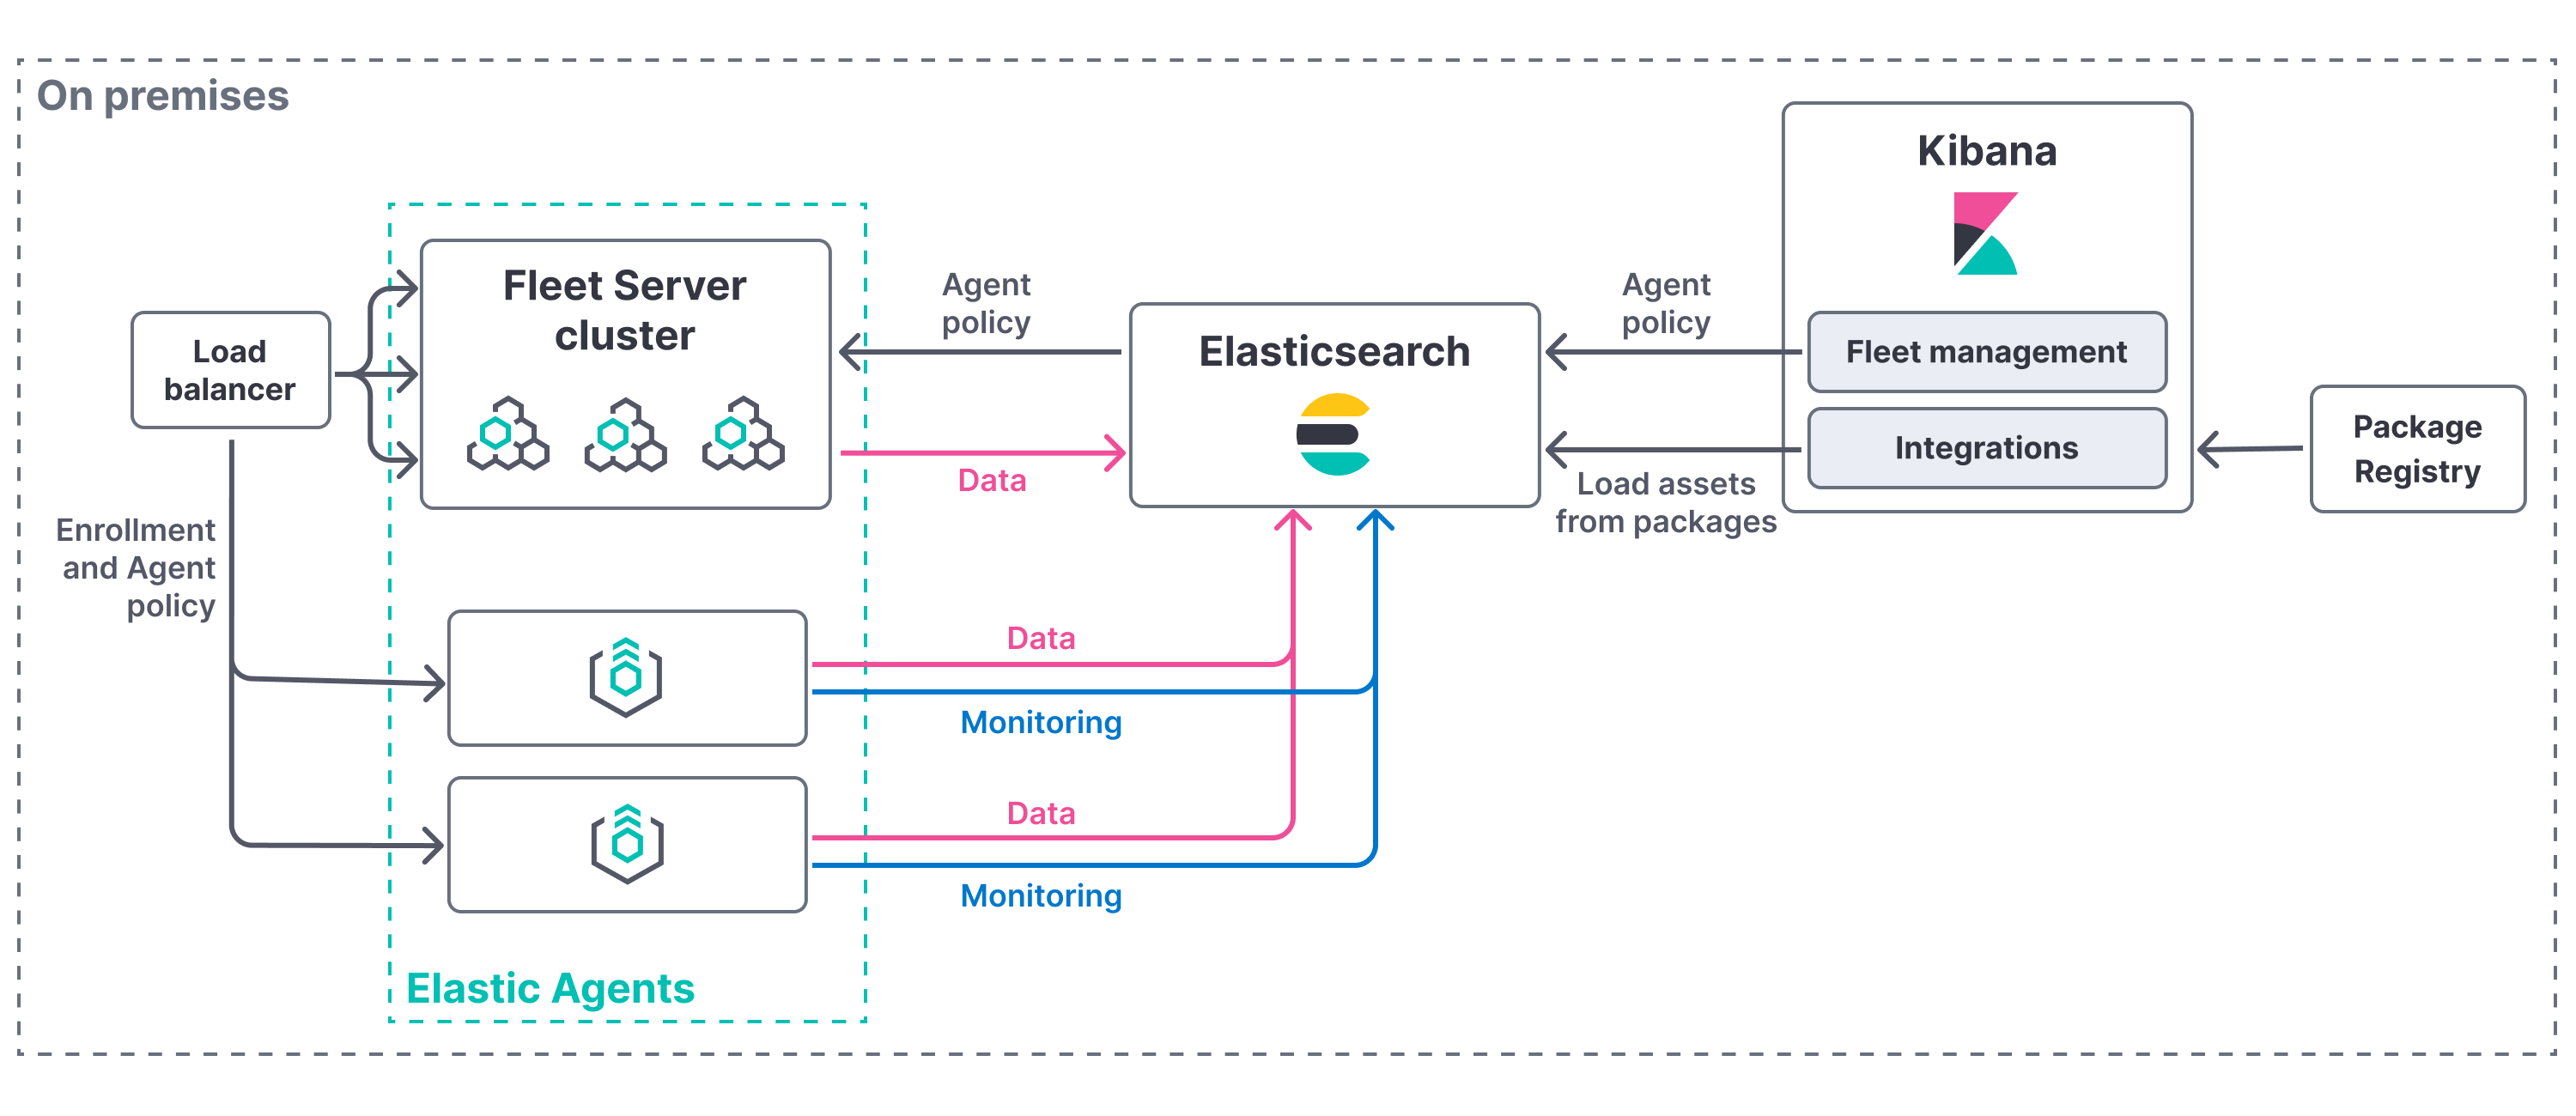
\includegraphics[width=\columnwidth]{fleet-agents.png} 
    \caption{Figura 4.3 - Funzionamento Elastic Agents e Fleet}
\end{figure}
La figura 4.3 mostra l'architettura generale di gestione degli agenti tramite \emph{Fleet}. Gli \emph{Elastic Agents} installati sull'applicazione comunicano con il \emph{Fleet Server} per ricevere le \emph{policy} di configurazione e inviare i dati raccolti a \emph{Elasticsearch} per la visualizzazione in \emph{Kibana}.   
\vspace{1em}

\subsection*{OpenTelemetry}
OpenTelemetry\footcite{site:opentelemetry} è un progetto \emph{open source} che fornisce un insieme di \gls{apig}, librerie e strumenti per la raccolta di dati di telemetria da applicazioni e servizi. L'obiettivo di OpenTelemetry è standardizzare la raccolta e l'esportazione di dati di telemetria mediante l'\gls{otlp}, facilitando l'integrazione con diversi sistemi di monitoraggio e analisi, tra cui l'Elastic Stack. OpenTelemetry supporta vari linguaggi di programmazione e offre un'architettura che consente agli sviluppatori di personalizzare la raccolta dei dati in base alle esigenze specifiche delle loro applicazioni.
\begin{figure}[H] 
    \centering 
    
\includegraphics[width=4cm]{/logos/OpenTelemetry.png} 
    \caption{Figura 4.4 - OpenTelemetry}
\end{figure}

\vspace{1em}

\subsection*{Elastic APM e APM Server}
Elastic APM\footcite{site:apm} è una soluzione di monitoraggio delle prestazioni applicative sviluppata da \emph{Elastic}, progettata per tracciare e analizzare le prestazioni delle applicazioni in tempo reale. Elastic APM consente di identificare colli di bottiglia, errori e problemi di latenza, fornendo una visione dettagliata del comportamento dell'applicazione attraverso tracce distribuite, metriche e log. \\
L'APM Server è un componente di Elastic APM che funge da punto di raccolta per i dati di telemetria inviati dagli agenti APM integrati nelle applicazioni. L'APM Server elabora questi dati e li invia a \emph{Elasticsearch} per l'indicizzazione, consentendo agli utenti di visualizzare le informazioni tramite \emph{Kibana}.
\begin{figure}[H] 
    \centering 
    
\includegraphics[width=4cm]{/logos/ElasticAPM.png} 
    \caption{Figura 4.5 - Elastic APM}
\end{figure}

\vspace{1em}

\subsection*{RUM Agent e Synthetic Monitoring}
Il RUM Agent (Real User Monitoring Agent)\footcite{site:rum-js} di Elastic APM, nel contesto del progetto di monitoraggio di \emph{PetClinic} è una libreria \emph{JavaScript} che consente di monitorare le prestazioni dell'applicazione \emph{web} dal punto di vista dell'utente finale. Integrando il RUM Agent nelle pagine web, è possibile raccogliere dati sulle interazioni degli utenti, i tempi di caricamento delle pagine e altri eventi significativi. Questi dati vengono inviati all'APM Server per l'analisi e la visualizzazione tramite Kibana. \\
Il Synthetic Monitoring\footcite{site:synthetic}, invece, utilizza \emph{script} automatizzati per simulare le interazioni degli utenti con l'applicazione web, consentendo di testare la disponibilità e le prestazioni da diverse località geografiche. Questa tecnica aiuta a identificare problemi prima che impattino sugli utenti reali, offrendo uno sguardo sulle prestazioni dell'applicazione.


\newpage
\subsection{Linguaggi di programmazione}
\subsection*{Python}
Python\footcite{site:python} è un linguaggio di programmazione ad alto livello, ampiamente utilizzato in vari ambiti, tra cui lo sviluppo web, l'analisi dei dati, l'intelligenza artificiale e l'automazione. Python è dotato di una vasta libreria standard e di un ecosistema ricco di pacchetti e framework che ne estendono le funzionalità e lo rendono un linguaggio versatile e potente. In questo progetto Python è stato utilizzato principalmente per la creazione di script di automazione tramite Selenium, al fine di eseguire test automatizzati sull'applicazione \emph{web PetClinic}.
\begin{figure}[H] 
    \centering 
    
\includegraphics[width=4cm]{/logos/Python_logonormal.png} 
    \caption{Figura 4.6 - Python}
\end{figure}

\vspace{1em}

\subsection*{JavaScript}
JavaScript\footcite{site:javascript} è un linguaggio di programmazione interpretato, utilizzato per lo sviluppo di applicazioni \emph{web} lato \emph{client} che consente di creare interfacce utente interattive e dinamiche. Nel contesto del progetto di monitoraggio di \emph{PetClinic}, JavaScript è stato utilizzato per integrare il RUM Agent di Elastic APM, permettendo la raccolta di dati sulle prestazioni dell'applicazione dal punto di vista dell'utente finale.
\begin{figure}[H] 
    \centering 
    
\includegraphics[width=4cm]{/logos/javascript.png} 
    \caption{Figura 4.7 - JavaScript}
\end{figure}

\vspace{1em}

\subsection*{Java}
Java\footcite{site:java} è un linguaggio di programmazione ad alto livello, orientato agli oggetti, ampiamente utilizzato nel mondo dello sviluppo software. OpenTelemetry fornisce un agente APM specifico per Java, che consente di monitorare le prestazioni di \emph{backend} dell'applicazione \emph{PetClinic} in modo dettagliato integrando l'agente Java nel codice dell'applicazione.
\begin{figure}[H] 
    \centering 
    
\includegraphics[width=4cm]{/logos/java.png} 
    \caption{Figura 4.8 - Java}
\end{figure}


\newpage
\subsection{Framework e librerie}
\subsection*{Node.js}
Node.js\footcite{site:nodejs} è utilizzato in PetClinic lato server per eseguire codice JavaScript. Funge da intermediario per le richieste tra il client e il server, gestendo operazioni asincrone e migliorando le prestazioni complessive dell'applicazione web.
\begin{figure}[H] 
    \centering 
    
\includegraphics[width=4cm]{/logos/nodeJS.png} 
    \caption{Figura 4.9 - Node.js}
\end{figure}

\vspace{1em}

\subsection*{Spring Boot}
Spring Boot\footcite{site:spring} è il framework principale utilizzato per sviluppare l'applicazione \emph{PetClinic}. Fornisce un ambiente di sviluppo semplificato per la creazione di applicazioni \emph{Java} basate su \emph{Spring}, offrendo funzionalità integrate per la gestione delle dipendenze, la configurazione automatica e il supporto per vari moduli come \emph{Spring MVC}, \emph{Spring Data} e \emph{Spring Security}.
\begin{figure}[H] 
    \centering 
    
\includegraphics[width=4cm]{/logos/spring.png} 
    \caption{Figura 4.10 - Spring}
\end{figure}

\vspace{1em}

\subsection*{Selenium}
Selenium\footcite{site:selenium} è un \emph{framework open source} utilizzato per l'automazione dei test delle applicazioni \emph{web}. Consente di simulare le interazioni degli utenti con il \emph{browser}, eseguendo test funzionali e di regressione in modo automatizzato. Selenium supporta diversi linguaggi di programmazione, tra cui \emph{Java}, \emph{Python} e \emph{JavaScript} e può essere integrato con vari strumenti di \emph{testing} e \emph{framework} di sviluppo. Durante il progetto è stata utilizzata la libreria Selenium per \emph{Python} per creare \emph{script} di test automatizzati che simulano le azioni degli utenti sull'applicazione \emph{PetClinic}.
\begin{figure}[H] 
    \centering 
    
\includegraphics[width=4cm]{/logos/selenium.png} 
    \caption{Figura 4.11 - Selenium}
\end{figure}


\newpage
\subsection{Strumenti di sviluppo}
\subsection*{VSCode}
Visual Studio Code (VSCode)\footcite{site:vscode} è un editor di codice sorgente sviluppato da Microsoft. Supporta una vasta gamma di linguaggi di programmazione e offre diverse funzionalità avanzate come il debugging integrato, il controllo della versione tramite \emph{Git} e un \emph{marketplace} ricco di estensioni.
\begin{figure}[H] 
    \centering 
    
\includegraphics[width=4cm]{/logos/vscode.png} 
    \caption{Figura 4.12 - VSCode}
\end{figure}


\newpage
\subsection{Database}
\subsection*{MySQL}
MySQL\footcite{site:mysql} è un sistema di gestione di \emph{database} relazionali \emph{open source}, ampiamente utilizzato per la memorizzazione e la gestione dei dati in applicazioni \emph{web} e aziendali. MySQL supporta il linguaggio \gls{sqlg}\glsfirstoccur per l'interrogazione e la manipolazione dei dati, offrendo funzionalità avanzate come transazioni, indicizzazione e replicazione. Nel contesto dell'applicazione \emph{PetClinic}, MySQL viene utilizzato come \emph{database} principale per archiviare le informazioni relative agli utenti, agli animali domestici, alle visite veterinarie e ad altri dati pertinenti all'applicazione.
\begin{figure}[H] 
    \centering 
    
\includegraphics[width=4cm]{/logos/Mysql_barattolo.png} 
    \caption{Figura 4.13 - MySQL}
\end{figure}


\newpage
\section{Criteri di scelta della soluzione}
\label{sec:criteri-scelta-soluzione}
Le principali motivazioni che hanno guidato la scelta della soluzione di monitoraggio basata su \emph{Elastic Stack} e \emph{OpenTelemetry} sono:
\begin{itemize}
    \item \textbf{Open source e flessibilità:} entrambe le tecnologie sono open source, consentendo una maggiore personalizzazione e adattabilità alle esigenze specifiche del progetto;
    \item \textbf{Scalabilità:} la soluzione è progettata per gestire grandi volumi di dati in ambienti distribuiti, garantendo prestazioni elevate anche con l'aumento del carico di lavoro;
    \item \textbf{Ecosistema completo:} \emph{Elastic Stack} offre un ecosistema completo per la raccolta, l'analisi e la visualizzazione dei dati, semplificando la gestione del sistema di monitoraggio;
    \item \textbf{Requisiti aziendali:} la scelta è stata influenzata dalla necessità di integrare il sistema di monitoraggio con l'infrastruttura esistente dell'azienda, che già utilizza componenti dell'\emph{Elastic Stack};
    \item \textbf{Comunità attiva:} entrambe le tecnologie vantano una comunità di sviluppatori attiva e in crescita, che contribuisce al miglioramento continuo delle piattaforme e fornisce supporto agli utenti.
\end{itemize}


\section{Integrazione con l'ambiente esistente}
\label{sec:integrazione-ambiente-esistente}
L'integrazione della soluzione di monitoraggio è stata progettata tenendo conto delle specifiche dell'ambiente tecnico aziendale, basato su infrastrutture \emph{Linux} e containerizzazione tramite \emph{Docker}. \\
Tutti i componenti dell'\emph{Elastic Stack} sono stati distribuiti in un ambiente isolato, mantenendo la compatibilità con le versioni approvate dall'azienda. \\
La comunicazione tra l'applicazione \emph{web PetClinic} e il sistema di osservabilità avviene tramite l'agente \emph{OpenTelemetry Java}, che esporta i dati di telemetria verso l'\emph{Elastic APM Server} gestito da \emph{Fleet}. 
L'approccio adottato permette un'integrazione trasparente con l'ambiente esistente, garantendo la scalabilità del sistema e la possibilità di estendere la soluzione ad altri servizi o applicazioni monitorate nel futuro.

%\section{Ciclo di vita del software}
%\label{sec:ciclo-vita-software}

%\section{Progettazione}
%\label{sec:progettazione}

%\subsubsection{Namespace 1} %**************************
%Descrizione namespace 1.

%\begin{namespacedesc}
    %\classdesc{Classe 1}{Descrizione classe 1}
    %\classdesc{Classe 2}{Descrizione classe 2}
%\end{namespacedesc}


%\section{Design Pattern utilizzati}

%\section{Codifica}
